\documentclass[
  DIV=calc,
  parskip=half,
  %headings=standardclasses,
  headsepline=true
]{scrartcl}

\usepackage[utf8]{inputenc}
\usepackage[T1]{fontenc}
\usepackage[lining]{libertine}
\usepackage{textcomp}
\usepackage[varqu,varl,scaled=0.95]{inconsolata}
\usepackage{amsthm}
\usepackage[libertine,vvarbb,libaltvw,liby]{newtxmath}
\usepackage[scr=rsfso]{mathalfa}
\usepackage{bm}
\useosf
\usepackage{microtype}
\UseMicrotypeSet[protrusion]{basicmath} % disable protrusion for tt fonts

$if(lang)$
\usepackage[
  $for(babel-otherlangs)$$babel-otherlangs$,$endfor$%
  main=$babel-lang$
]{babel}
$endif$

\setlength\parindent{0in}

% fix for pandoc 1.14
\providecommand{\tightlist}{%
  \setlength{\itemsep}{1em}\setlength{\parskip}{0.15em}}

% TABLES AND LISTS
\usepackage{enumitem}
\usepackage{longtable}
\usepackage{booktabs}

\usepackage{graphicx}

% Capheight
\newlength{\capheight}
% Create the reference text for measures
\settoheight{\capheight}{B}

% HEADERS AND FOOTERS
\usepackage{scrlayer-scrpage}
\pagestyle{scrheadings}
\lohead[]{CV}
\rohead[]{Larsson, J}

% HYPERREF
\usepackage[hyperfootnotes=false]{hyperref}
\PassOptionsToPackage{usenames,dvipsnames}{xcolor}
\PassOptionsToPackage{hyphens}{url}
\hypersetup{
  unicode=true,
  pdftitle={CV},
  pdfauthor={Johan Larsson},
  colorlinks=true,
  linkcolor=Maroon,
  citecolor=Blue,
  urlcolor=Blue,
  breaklinks=true
}
\usepackage[anythingbreaks]{breakurl}

\usepackage{tikz}
\usepackage{tabularx}

\urlstyle{same}

% TITLEPAGE
\date{\today}

\title{Johan Larsson}
%\subtitle{CV}
%\author{CV}

%\addtokomafont{subtitle}{\huge\itshape}
%\addtokomafont{author}{\huge\itshape}

\setlist[description]{
  font=\rmfamily\footnotesize,
  align=parleft,
  labelwidth=5em,
  leftmargin=5em,
  labelindent=0em,
  labelsep=0em
}

% Fix \latex
\let\textLaTeX\LaTeX
\renewcommand*{\LaTeX}{\textLaTeX}

% BEGIN DOCUMENT
\begin{document}

\begin{titlepage}
\end{titlepage}

\begin{minipage}{.5\textwidth}

{\itshape \large \textcolor{Gray}{CV}}
\medskip

\noindent {\Huge \sffamily \bfseries Johan Larsson}

\noindent {\large \today}
\end{minipage}%
\begin{minipage}{0.5\textwidth}
  \raggedleft
  \begin{tikzpicture}
        \begin{scope}
          \clip [rounded corners=1cm] (0,0) rectangle coordinate (centerpoint) (2,2cm);
          \node [inner sep=0pt] at (centerpoint) {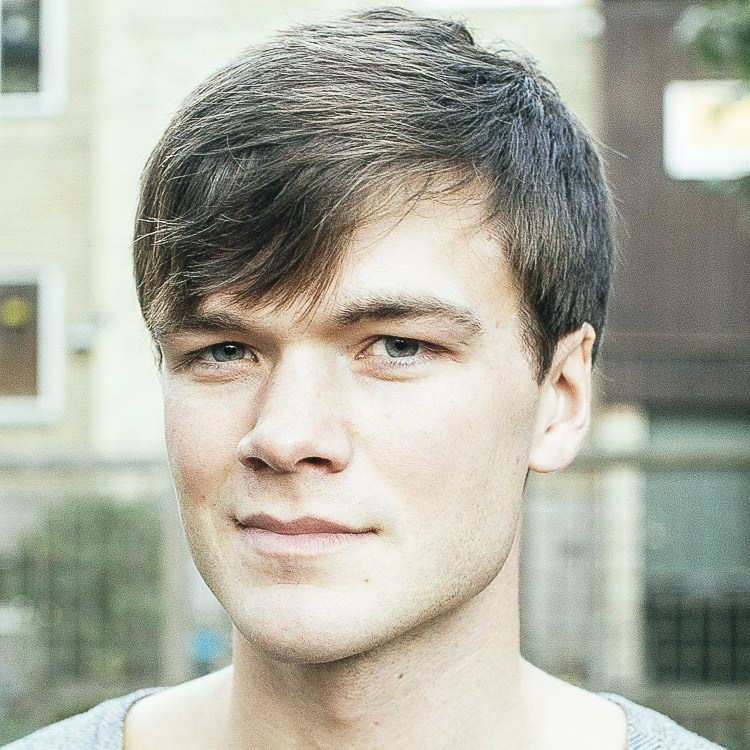
\includegraphics[width=2cm, height=2cm]{assets/profilbild}};
        \end{scope}
  \end{tikzpicture}
\end{minipage}

\vskip 1.5\baselineskip

\begin{minipage}{.5\textwidth}
\small
\itshape
\noindent Mellanvångsvägen 2B\\
22358 Lund, Sweden\\
\href{mailto:mail@larssonjohan.com}{mail@larssonjohan.com}\\
+46 730353836

\end{minipage}%
\begin{minipage}{0.5\textwidth}
\raggedleft\itshape\small
\href{https://larssonjohan.com}{larssonjohan.com}\\
\href{http://orcid.org/0000-0002-4029-5945}{
\includegraphics[height=\capheight]{assets/orcid.pdf} orcid.org/0000-0002-4029-5945}\\
\href{https://www.researchgate.net/profile/Johan_Larsson7}{
\includegraphics[height=\capheight]{assets/researchgate.pdf} researchgate.net/profile/Johan\_Larsson7}\\
\href{http://publons.com/a/1299032}{
\includegraphics[height=\capheight]{assets/publons.pdf} publons.com/a/1299032}]
\end{minipage}

\tableofcontents

$body$

\end{document}
